
%% IAENG_pub.tex 2010/08/30
%% It is based on the bare_jrnl.tex V1.3 2007/01/11 by Michael Shell
%% see http://www.michaelshell.org/
%% for current contact information.
%%
%% This is a skeleton file demonstrating the use of IAENGtran.cls
%% (requires IAENGtran.cls version 1.7 or later) with an IAENG journal/conference paper.
%%
%% Support sites:
%% http://www.michaelshell.org/tex
%% http://www.ctan.org/tex-archive/macros/latex/contrib/IEEEtran/

% *** Authors should verify (and, if needed, correct) their LaTeX system  ***
% *** with the testflow diagnostic prior to trusting their LaTeX platform ***
% *** with production work. IAENG's font choices can trigger bugs that do  ***
% *** not appear when using other class files.                            ***
% The testflow support page is at:
% http://www.michaelshell.org/tex/testflow/


%%*************************************************************************
%% Legal Notice:
%% This code is offered as-is without any warranty either expressed or
%% implied; without even the implied warranty of MERCHANTABILITY or
%% FITNESS FOR A PARTICULAR PURPOSE!
%% User assumes all risk.
%% In no event shall IAENG or any contributor to this code be liable for
%% any damages or losses, including, but not limited to, incidental,
%% consequential, or any other damages, resulting from the use or misuse
%% of any information contained here.
%%
%% All comments are the opinions of their respective authors and are not
%% necessarily endorsed by the IAENG.
%%
%% This work is distributed under the LaTeX Project Public License (LPPL)
%% ( http://www.latex-project.org/ ) version 1.3, and may be freely used,
%% distributed and modified. A copy of the LPPL, version 1.3, is included
%% in the base LaTeX documentation of all distributions of LaTeX released
%% 2003/12/01 or later.
%% Retain all contribution notices and credits.
%% ** Modified files should be clearly indicated as such, including  **
%% ** renaming them and changing author support contact information. **
%%
%%*************************************************************************

% Note that the a4paper option is mainly intended so that authors in
% countries using A4 can easily print to A4 and see how their papers will
% look in print - the typesetting of the document will not typically be
% affected with changes in paper size (but the bottom and side margins will).
% Use the testflow package mentioned above to verify correct handling of
% both paper sizes by the user's LaTeX system.
%
% Also note that the "draftcls" or "draftclsnofoot", not "draft", option
% should be used if it is desired that the figures are to be displayed in
% draft mode.
%
\documentclass[journal]{IAENGtran}
%
% If IAENGtran.cls has not been installed into the LaTeX system files,
% manually specify the path to it like:
% \documentclass[journal]{../sty/IAENGtran}





% Some very useful LaTeX packages include:
% (uncomment the ones you want to load)


% *** MISC UTILITY PACKAGES ***
%
%\usepackage{ifpdf}
% Heiko Oberdiek's ifpdf.sty is very useful if you need conditional
% compilation based on whether the output is pdf or dvi.
% usage:
% \ifpdf
%   % pdf code
% \else
%   % dvi code
% \fi
% The latest version of ifpdf.sty can be obtained from:
% http://www.ctan.org/tex-archive/macros/latex/contrib/oberdiek/
% Also, note that IAENGtran.cls V1.7 and later provides a builtin
% \ifCLASSINFOpdf conditional that works the same way.
% When switching from latex to pdflatex and vice-versa, the compiler may
% have to be run twice to clear warning/error messages.






% *** CITATION PACKAGES ***
%
%\usepackage{cite}
% cite.sty was written by Donald Arseneau
% V1.6 and later of IAENGtran pre-defines the format of the cite.sty package
% \cite{} output to follow that of IAENG. Loading the cite package will
% result in citation numbers being automatically sorted and properly
% "compressed/ranged". e.g., [1], [9], [2], [7], [5], [6] without using
% cite.sty will become [1], [2], [5]--[7], [9] using cite.sty. cite.sty's
% \cite will automatically add leading space, if needed. Use cite.sty's
% noadjust option (cite.sty V3.8 and later) if you want to turn this off.
% cite.sty is already installed on most LaTeX systems. Be sure and use
% version 4.0 (2003-05-27) and later if using hyperref.sty. cite.sty does
% not currently provide for hyperlinked citations.
% The latest version can be obtained at:
% http://www.ctan.org/tex-archive/macros/latex/contrib/cite/
% The documentation is contained in the cite.sty file itself.






% *** GRAPHICS RELATED PACKAGES ***
%
\ifCLASSINFOpdf
   \usepackage[pdftex]{graphicx}
  % declare the path(s) where your graphic files are
  % \graphicspath{{../pdf/}{../jpeg/}}
  % and their extensions so you won't have to specify these with
  % every instance of \includegraphics
   \DeclareGraphicsExtensions{.pdf,.jpeg,.png}
\else
  % or other class option (dvipsone, dvipdf, if not using dvips). graphicx
  % will default to the driver specified in the system graphics.cfg if no
  % driver is specified.
   \usepackage[dvips]{graphicx}
  % declare the path(s) where your graphic files are
  % \graphicspath{{../eps/}}
  % and their extensions so you won't have to specify these with
  % every instance of \includegraphics
   \DeclareGraphicsExtensions{.eps}
\fi
% graphicx was written by David Carlisle and Sebastian Rahtz. It is
% required if you want graphics, photos, etc. graphicx.sty is already
% installed on most LaTeX systems. The latest version and documentation can
% be obtained at:
% http://www.ctan.org/tex-archive/macros/latex/required/graphics/
% Another good source of documentation is "Using Imported Graphics in
% LaTeX2e" by Keith Reckdahl which can be found as epslatex.ps or
% epslatex.pdf at: http://www.ctan.org/tex-archive/info/
%
% latex, and pdflatex in dvi mode, support graphics in encapsulated
% postscript (.eps) format. pdflatex in pdf mode supports graphics
% in .pdf, .jpeg, .png and .mps (metapost) formats. Users should ensure
% that all non-photo figures use a vector format (.eps, .pdf, .mps) and
% not a bitmapped formats (.jpeg, .png). IAENG frowns on bitmapped formats
% which can result in "jaggedy"/blurry rendering of lines and letters as
% well as large increases in file sizes.
%
% You can find documentation about the pdfTeX application at:
% http://www.tug.org/applications/pdftex





% *** MATH PACKAGES ***
%
%\usepackage[cmex10]{amsmath}
% A popular package from the American Mathematical Society that provides
% many useful and powerful commands for dealing with mathematics. If using
% it, be sure to load this package with the cmex10 option to ensure that
% only type 1 fonts will utilized at all point sizes. Without this option,
% it is possible that some math symbols, particularly those within
% footnotes, will be rendered in bitmap form which will result in a
% document that can not be IAENG compliant!
%
% Also, note that the amsmath package sets \interdisplaylinepenalty to 10000
% thus preventing page breaks from occurring within multiline equations. Use:
%\interdisplaylinepenalty=2500
% after loading amsmath to restore such page breaks as IAENGtran.cls normally
% does. amsmath.sty is already installed on most LaTeX systems. The latest
% version and documentation can be obtained at:
% http://www.ctan.org/tex-archive/macros/latex/required/amslatex/math/





% *** SPECIALIZED LIST PACKAGES ***
%
%\usepackage{algorithmic}
% algorithmic.sty was written by Peter Williams and Rogerio Brito.
% This package provides an algorithmic environment for describing algorithms.
% You can use the algorithmic environment in-text or within a figure
% environment to provide for a floating algorithm. Do NOT use the algorithm
% floating environment provided by algorithm.sty (by the same authors) or
% algorithm2e.sty (by Christophe Fiorio) as IAENG does not use dedicated
% algorithm float types and packages that provide these will not provide
% correct IAENG style captions. The latest version and documentation of
% algorithmic.sty can be obtained at:
% http://www.ctan.org/tex-archive/macros/latex/contrib/algorithms/
% There is also a support site at:
% http://algorithms.berlios.de/index.html
% Also of interest may be the (relatively newer and more customizable)
% algorithmicx.sty package by Szasz Janos:
% http://www.ctan.org/tex-archive/macros/latex/contrib/algorithmicx/




% *** ALIGNMENT PACKAGES ***
%
%\usepackage{array}
% Frank Mittelbach's and David Carlisle's array.sty patches and improves
% the standard LaTeX2e array and tabular environments to provide better
% appearance and additional user controls. As the default LaTeX2e table
% generation code is lacking to the point of almost being broken with
% respect to the quality of the end results, all users are strongly
% advised to use an enhanced (at the very least that provided by array.sty)
% set of table tools. array.sty is already installed on most systems. The
% latest version and documentation can be obtained at:
% http://www.ctan.org/tex-archive/macros/latex/required/tools/


%\usepackage{mdwmath}
%\usepackage{mdwtab}
% Also highly recommended is Mark Wooding's extremely powerful MDW tools,
% especially mdwmath.sty and mdwtab.sty which are used to format equations
% and tables, respectively. The MDWtools set is already installed on most
% LaTeX systems. The lastest version and documentation is available at:
% http://www.ctan.org/tex-archive/macros/latex/contrib/mdwtools/


% IAENGtran contains the IAENGeqnarray family of commands that can be used to
% generate multiline equations as well as matrices, tables, etc., of high
% quality.


%\usepackage{eqparbox}
% Also of notable interest is Scott Pakin's eqparbox package for creating
% (automatically sized) equal width boxes - aka "natural width parboxes".
% Available at:
% http://www.ctan.org/tex-archive/macros/latex/contrib/eqparbox/





% *** SUBFIGURE PACKAGES ***
%\usepackage[tight,footnotesize]{subfigure}
% subfigure.sty was written by Steven Douglas Cochran. This package makes it
% easy to put subfigures in your figures. e.g., "Figure 1a and 1b". For IAENG
% work, it is a good idea to load it with the tight package option to reduce
% the amount of white space around the subfigures. subfigure.sty is already
% installed on most LaTeX systems. The latest version and documentation can
% be obtained at:
% http://www.ctan.org/tex-archive/obsolete/macros/latex/contrib/subfigure/
% subfigure.sty has been superceeded by subfig.sty.



%\usepackage[caption=false]{caption}
%\usepackage[font=footnotesize]{subfig}
% subfig.sty, also written by Steven Douglas Cochran, is the modern
% replacement for subfigure.sty. However, subfig.sty requires and
% automatically loads Axel Sommerfeldt's caption.sty which will override
% IAENGtran.cls handling of captions and this will result in nonIAENG style
% figure/table captions. To prevent this problem, be sure and preload
% caption.sty with its "caption=false" package option. This is will preserve
% IAENGtran.cls handing of captions. Version 1.3 (2005/06/28) and later
% (recommended due to many improvements over 1.2) of subfig.sty supports
% the caption=false option directly:
%\usepackage[caption=false,font=footnotesize]{subfig}
%
% The latest version and documentation can be obtained at:
% http://www.ctan.org/tex-archive/macros/latex/contrib/subfig/
% The latest version and documentation of caption.sty can be obtained at:
% http://www.ctan.org/tex-archive/macros/latex/contrib/caption/




% *** FLOAT PACKAGES ***
%
%\usepackage{fixltx2e}
% fixltx2e, the successor to the earlier fix2col.sty, was written by
% Frank Mittelbach and David Carlisle. This package corrects a few problems
% in the LaTeX2e kernel, the most notable of which is that in current
% LaTeX2e releases, the ordering of single and double column floats is not
% guaranteed to be preserved. Thus, an unpatched LaTeX2e can allow a
% single column figure to be placed prior to an earlier double column
% figure. The latest version and documentation can be found at:
% http://www.ctan.org/tex-archive/macros/latex/base/



%\usepackage{stfloats}
% stfloats.sty was written by Sigitas Tolusis. This package gives LaTeX2e
% the ability to do double column floats at the bottom of the page as well
% as the top. (e.g., "\begin{figure*}[!b]" is not normally possible in
% LaTeX2e). It also provides a command:
%\fnbelowfloat
% to enable the placement of footnotes below bottom floats (the standard
% LaTeX2e kernel puts them above bottom floats). This is an invasive package
% which rewrites many portions of the LaTeX2e float routines. It may not work
% with other packages that modify the LaTeX2e float routines. The latest
% version and documentation can be obtained at:
% http://www.ctan.org/tex-archive/macros/latex/contrib/sttools/
% Documentation is contained in the stfloats.sty comments as well as in the
% presfull.pdf file. Do not use the stfloats baselinefloat ability as IAENG
% does not allow \baselineskip to stretch. Authors submitting work to the
% IAENG should note that IAENG rarely uses double column equations and
% that authors should try to avoid such use. Do not be tempted to use the
% cuted.sty or midfloat.sty packages (also by Sigitas Tolusis) as IAENG does
% not format its papers in such ways.


%\ifCLASSOPTIONcaptionsoff
%  \usepackage[nomarkers]{endfloat}
% \let\MYoriglatexcaption\caption
% \renewcommand{\caption}[2][\relax]{\MYoriglatexcaption[#2]{#2}}
%\fi
% endfloat.sty was written by James Darrell McCauley and Jeff Goldberg.
% This package may be useful when used in conjunction with IAENGtran.cls'
% captionsoff option. Some IAENG journals/societies require that submissions
% have lists of figures/tables at the end of the paper and that
% figures/tables without any captions are placed on a page by themselves at
% the end of the document. If needed, the draftcls IAENGtran class option or
% \CLASSINPUTbaselinestretch interface can be used to increase the line
% spacing as well. Be sure and use the nomarkers option of endfloat to
% prevent endfloat from "marking" where the figures would have been placed
% in the text. The two hack lines of code above are a slight modification of
% that suggested by in the endfloat docs (section 8.3.1) to ensure that
% the full captions always appear in the list of figures/tables - even if
% the user used the short optional argument of \caption[]{}.
% IAENG papers do not typically make use of \caption[]'s optional argument,
% so this should not be an issue. A similar trick can be used to disable
% captions of packages such as subfig.sty that lack options to turn off
% the subcaptions:
% For subfig.sty:
% \let\MYorigsubfloat\subfloat
% \renewcommand{\subfloat}[2][\relax]{\MYorigsubfloat[]{#2}}
% For subfigure.sty:
% \let\MYorigsubfigure\subfigure
% \renewcommand{\subfigure}[2][\relax]{\MYorigsubfigure[]{#2}}
% However, the above trick will not work if both optional arguments of
% the \subfloat/subfig command are used. Furthermore, there needs to be a
% description of each subfigure *somewhere* and endfloat does not add
% subfigure captions to its list of figures. Thus, the best approach is to
% avoid the use of subfigure captions (many IAENG journals avoid them anyway)
% and instead reference/explain all the subfigures within the main caption.
% The latest version of endfloat.sty and its documentation can obtained at:
% http://www.ctan.org/tex-archive/macros/latex/contrib/endfloat/
%
% The IAENGtran \ifCLASSOPTIONcaptionsoff conditional can also be used
% later in the document, say, to conditionally put the References on a
% page by themselves.





% *** PDF, URL AND HYPERLINK PACKAGES ***
%
%\usepackage{url}
% url.sty was written by Donald Arseneau. It provides better support for
% handling and breaking URLs. url.sty is already installed on most LaTeX
% systems. The latest version can be obtained at:
% http://www.ctan.org/tex-archive/macros/latex/contrib/misc/
% Read the url.sty source comments for usage information. Basically,
% \url{my_url_here}.





% *** Do not adjust lengths that control margins, column widths, etc. ***
% *** Do not use packages that alter fonts (such as pslatex).         ***
% There should be no need to do such things with IAENGtran.cls V1.6 and later.
% (Unless specifically asked to do so by the journal or conference you plan
% to submit to, of course. )


% correct bad hyphenation here
% \hyphenation{op-tical net-works semi-conduc-tor}


\begin{document}
%
% paper title
% can use linebreaks \\ within to get better formatting as desired
\title{An Explanation Method of Unfamiliar Tourist Spots based on Roles of User's Familiar Spots}
%
%
% author names and IAENG memberships
% note positions of commas and nonbreaking spaces ( ~ ) LaTeX will not break
% a structure at a ~ so this keeps an author's name from being broken across
% two lines.
% use \thanks{} to gain access to the first footnote area
% a separate \thanks must be used for each paragraph as LaTeX2e's \thanks
% was not built to handle multiple paragraphs
%

\author{Michael~Shell,~\IAENGmembership{Member,~IAENG,}
        John~Doe,~\IAENGmembership{Senior Member,~IAENG,}
        and~Jane~Doe,~\IAENGmembership{Fellow,~IAENG}% <-this % stops a space
\thanks{Manuscript received April XX, 20XX; revised June XX, 20XX. (Write the date on
which you submitted your paper for review.) This work was supported
in part by the U.S. Department of Commerce under Grant BS123456
(sponsor and financial support acknowledgment goes here). Paper
titles should be written in uppercase and lowercase letters, not all
uppercase. Avoid writing long formulas with subscripts in the title;
short formulas that identify the elements are fine.}
\thanks{M. Shell is with the Department
of Electrical and Computer Engineering, Georgia Institute of
Technology, Atlanta,
GA, 30332 USA e-mail: (see http://www.michaelshell.org/contact.html).}% <-this % stops a space
\thanks{J. Doe and J. Doe are with Anonymous University.}}% <-this % stops a space


% make the title area
\maketitle

\pagestyle{empty}
\thispagestyle{empty}

%%%%%%%%%%%%%%%%%%%%%%%%%%%%%%%%%%%%%%%%%%
%%%%%%%%%%%%%%%%%%%%%%%%%%%%%%%%%%%%%%%%%%
\begin{abstract}
%\boldmath

% 近年,観光スポットを決める時にWeb上の観光情報を活用して計画を立てることが多くなっている.
In recent years, when planning tourist spots, planning is often made by utilizing tourist information on the Web.
% しかし,ユーザが多くのエリアから訪問したいエリアを決めた上で,さらに自分のイメージに合う観光スポットを探すのは膨大な時間と労力を必要とする.
However, after deciding the area you want to visit from many areas, the user also needs enormous amount of time and effort to find tourist spots that match your image.
% また,ユーザが未訪問スポットに対して期待と不安を感じる場合がある.
In addition, there are cases where the user feels expectation and anxiety with respect to the unvisited spot.
% 本研究では,ユーザの未知なスポットに対する理解を支援するためには,既に訪問したことがある観光スポットの特徴を未訪問スポットにあてはめて理解を支援する説明手法を提案する.
In this research, in order to support understanding of users' unknown spots, we propose explanatory method that supports the understanding by fitting the features of tourist spots that have already visited to unvisited spots.
% 観光スポット自身の特徴を重視するため,各観光スポットの特徴抽出に,ユーザが入力した観光スポットのすべてのレビュー,対象エリアの観光スポットのすべてのレビューを使用する.
In order to emphasize the features of the tourist spots themselves, extraction of features of each tourist spot is done by work using all reviews of tourist spots entered by the user, all reviews of tourist spots in the target area.
% また,プロトタイプシステムを構築し,既訪問スポットと未訪問スポットとの説明情報の効果を検証する評価実験を行う.
We also conduct an evaluation experiment to construct the prototype system and verify the effect of the explanatory information between the visited spot and the unvisited spot.
\end{abstract}

%%%%%%%%%%%%%%%%%%%%%%%%%%%%%%%%%%%%%%%%%%
%%%%%%%%%%%%%%%%%%%%%%%%%%%%%%%%%%%%%%%%%%
\begin{IAENGkeywords}
% 観光スポット,理解支援,レビュー,コサイン類似度,TFIDF,調和平均
tourist spots, understanding support, reviews, cosine similarity, TFIDF, harmonic mean
\end{IAENGkeywords}

\IAENGpeerreviewmaketitle


%%%%%%%%%%%%%%%%%%%%%%%%%%%%%%%%%%%%%%%%%%
%%%%%%%%%%%%%%%%%%%%%%%%%%%%%%%%%%%%%%%%%%
\section{Introduction}
\label{sec:Introduction}
%%%%%%%%%%%%%%%%%%%%%%%%%%%%%%%%%%%%%%%%%%
%%%%%%%%%%%%%%%%%%%%%%%%%%%%%%%%%%%%%%%%%%
% 旅行先を決定する時,旅行者は観光スポット検索サイトや観光情報に関連する書籍を見て観光スポットを選び,旅行計画を立てる.
\IAENGPARstart{W}{hen} deciding the travel destination, the traveler selects tourist spots by planning a travel plan, watching tourist spots search sites and books related to tourist information.
% しかし,ユーザにとって訪問したいエリアを決定した後,さらにエリア内に数多く存在する観光スポットから,自身のイメージから外れない観光スポットを見つけることは容易ではない.
However, after deciding the area you want to visit from many areas,and further from their many tourist spots in the area is not easy to find.
% 行きたい観光スポットが決まっていない場合ではランキングやおすすめ情報を見て観光スポットを決めることが多くなると考えられる.
In the case where the tourist spots desired to go are not decided, it is considered that it is more likely to decide tourist spots by looking at ranking and recommendation information.
% この時,ユーザが選択した観光スポットに対するイメージが曖昧になるため不安を感じる場合がある.
At this time, the image for the tourist spots selected by the user becomes ambiguous, which may cause anxiety.


% 近年,観光業とソーシャルネットワーキングサービスの発展スピードが加速しており,体験した観光スポットに対するレビューを観光スポット検索サイトに投稿しているユーザが増加している.
In recent years, the speed of development of tourism industry and social networking service is accelerating, and the number of users who post reviews on tourist spots experienced to the tourist spot search site is increasing.
% さまざまな観光スポットを効果的に理解するためには,既存の情報をもとにして,未知な情報と既知な情報との対応関係を考えることが不可欠となる.
In order to effectively understand various tourist spots, it is essential to consider the correspondence between unknown information and existing information based on existing information.
% この考え方は,以前に経験した事柄(ベースと呼ぶ)を,現在直面している事柄あるいは問題(ターゲットと呼ぶ)にあてはめる類推に相当する.
This way of thinking is equivalent to analogy which applies to the things by previous experiences (called the base), or problems (called the target).
% たとえば,金沢の「にし茶屋街」という未知なスポットに対して既訪問の京都の「花見小路」と似ていると説明するとイメージの理解がしやすくすることがある.
For example, whereas unknown spots such as ``Kanazawa's Nisityayagai'', if you explain that it is similar to the already visited ``Kyoto Hanamikoj'', it may make it easier to understand the image.

% 本研究では,ユーザの未知なスポットに対する理解を支援するため,既に訪問したことがある観光スポットの特徴を未訪問スポットにあてはめて理解を支援する説明手法を提案する.
In this research, in order to support understanding of users' unknown spots, we propose explanatory method that supports the understanding by fitting the features of tourist spots that have already visited to unvisited spots.
% 具体的には,ユーザが入力した既訪問スポットと未訪問エリアから,レビュを用いて既訪問スポット内の各スポットの独特な特徴と未訪問エリア内の各スポットの独特な特徴を抽出し,比較を行って説明情報を提示する.
Specifically, from the already visited spot and the unvisited area entered by the user, we use the review to extract the unique features of each spot in the already visited spot and the unique features of each spot in the unvisited area, compare and present explanatory information.
% このプロトタイプシステムにより,ユーザが未訪問スポットに対する理解の支援を目指す.
With this prototype system, users aim to support understanding of unvisited spots.
% 図\ref{fig:Photo_Image}は提案手法の概念図である.
Fig. \ref{fig:Photo_Image} is a conceptual diagram of the proposed method.

% 本論文の構成は下記のとおりである.2節では関連研究について述べる.3節では提案手法の概要について述べる.4節では構築したプロトタイプシステムの効果を検証する評価実験と考察について述べる.最後に5節ではまとめと今後の課題について述べる.
The structure of this paper is as follows.
Section \ref{sec:Related Work} describes related research.
Section \ref{sec:An Explaination Method of Unfamiliar Tourist Spots} gives an overview of the proposed method.
Section \ref{sec:Evaluation Experiment} describes evaluation experiments and considerations to verify the effect of the constructed prototype system.
Section \ref{sec:Conclusions and Future Work} describes with conclusions and future work.

\begin{figure}[t]
  \begin{center}
    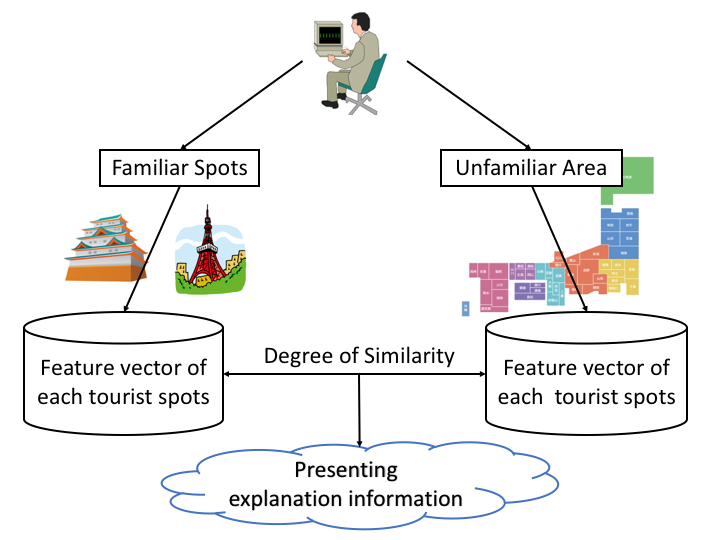
\includegraphics[clip,width=7.5cm,bb=0 0 720 540]{picture/Photo_Image_eng.png}
    % ユーザの既訪問スポットの位置づけに基づく未訪問スポット(エリア)の説明手法
    \caption{An explanation method of unfamiliar tourist spots based on roles of user's familiar spots}
    \label{fig:Photo_Image}
   \end{center}
\end{figure}


%%%%%%%%%%%%%%%%%%%%%%%%%%%%%%%%%%%%%%%%%%
%%%%%%%%%%%%%%%%%%%%%%%%%%%%%%%%%%%%%%%%%%
\section{Related Work}
\label{sec:Related Work}
%%%%%%%%%%%%%%%%%%%%%%%%%%%%%%%%%%%%%%%%%%
%%%%%%%%%%%%%%%%%%%%%%%%%%%%%%%%%%%%%%%%%%
\subsection{Research using user history}
\label{subsec:Research using user history}

% ユーザの体験履歴を利用した検索や推薦システムに関する研究が数多く発表されている.
Many researches on retrieval and recommendation system using the user's experience history have been published.
% 倉島ら\cite{Codd01}は,Flickrに投稿された写真のジオタグ情報を人々の旅行履歴として利用した旅行ルート推薦手法を提案した.
Kurashima et al.\cite{Codd01} proposed a travel route recommendation method using geotag information of photos posted to Flickr as a travel history of people.
% この手法では,ユーザの現在地から行きやすい場所とユーザの興味に合致した場所に移動しやすいと仮定し,行動モデルを生成している.
In this method, it is assumed that it is easy to move from a user's present location to a place easily accessible to the user's interest, and a behavior model is generated.
% ユーザのジオタグ付き写真集合は,時間情報でソートすると個人の旅行履歴とみなすことができると考え,ジオタグ情報を利用してユーザの行動モデルを生成している.
That geotagged photo aggregation of users can be regarded as personal travel history when sorted by time information, and we generate user behavior model using geotag information.
% 北村らは\cite{Codd02},一般的な物体認識を用いて,過去の個人旅行写真から旅行計画のユーザの嗜好を推定することに基づいて観光地を推薦する方法を提案した.
Kitamura et al.\cite{Codd02} proposed a method of recommending sightseeing spots based on estimating user's preferences of travel plan from past personal travel photographs using general object recognition.
% 物体認識システムを用いて,写真で撮った被写体情報のキーワードを取得し,グラフ視覚化技術によってキーワードの共起を表現した.
Using an object recognition system to acquire keywords of subject information taken in the photos and represented the co-occurrence of the keywords by a graph visualization technique.
% また,グラフの視覚化技術に基づいて旅行写真付きのグラフを視覚化するユーザインターフェイスを紹介した.
In addition, present a user interface that visualizes a graph with travel photos based on our graph visualization technique.
% Chengらは\cite{Codd03},自由に利用できるコミュニティ寄稿の写真を活用して,パーソナライズされた旅行のおすすめに焦点を当て,特定のユーザープロファイルまたは属性を考慮し,パーソナライズされた旅行の推奨を行うことを提案した.
Cheng et al.\cite{Codd03} used photographs of freely available community contributions to focus on personalized trip recommendations, considering specific user profiles or attributes, suggested to consider personalized travel recommendations.

%%%%%%%%%%%%%%%%%%%%%%%%%%%%%%%%%%%%%%%%%%
\subsection{Research on analogy}
\label{subsec:Research on analogy}

% 類推は創造的思考に貢献すると指摘されてた\cite{Codd04}.
Analogies were pointed out as contributing to creative thinking\cite{Codd04}.
% 既知の知識(ベースと呼ぶ)から概念(ターゲットと呼ぶ)を獲得するときに類推思考が働くとされる\cite{Codd05}.
Analogical thinking works when acquiring a concept (called the target) from known knowledge (called the bases)\cite{Codd05}.
% 類推に関する研究の多くは,ベースとなる学習データとターゲットとなる問題が与えられ,物事の特徴を問題の特徴にマッピングして問題を解決するもの\cite{Codd06}である.
Many of the researches on analogy are given the base learning data and targeted problems, and the problems are solved by mapping the features of things to the characteristics of the problem\cite{Codd06}.
% Gickらは,不確定な問題の解を見つけるためのガイドとして,異種ドメイン間の類推の使用を調査するように設計した.
Gick et al. designed to investigate the use of analogies between disparate domains as a guide to finding solutions for an ill-defined problem.
% 学習データの与え方や機能について研究したもの\cite{Codd07}や,認知的な熟達度に応じて問題を解決するかどうかを明らかにしたもの\cite{Codd08}がある.
Some studied about how to give learning data and functions\cite{Codd07}, and clarified whether to solve the problem depending on the degree of cognitive proficiency\cite{Codd08}.
% これらを含む従来研究の多くにおいては,類推に用いるベースとターゲットを与えたうえで,一定の手順に従って問題解決を行っている.
In many of the conventional research including these, after giving bases and targets for analogy, we solve problems according to a certain procedure.
% また,構造の類似性には3種類あり,特徴の共有数で決まる「対象レベルの類似性」,ベースに存在する関係とターゲットに存在する関係の共有度に基づく「関係レベルの類似性」,および題の解法あるいは目標レベルでの類似性である「プラグマティックな類似性」とがある\cite{Codd05},\cite{Codd09}.
There are three types of structural similarities``similarity of object level'' determined by the number of shared features, ``relationship similarity'' based on the degree of sharedness of relationships existing in the base and the relationship existing in the base, and similarity in the title solution or target level There is a certain ``pragmatic similarity''\cite{Codd05},\cite{Codd09}.

% 従来のユーザの体験履歴を利用する手法では,履歴写真のジオタグ情報を分析し,ユーザの嗜好とする研究が多く行われている.
In the conventional method of using the user's experience history, many researches that analyze the geotag information of the history photograph and make it user's preference are performed.
% また,類推技術に関して学習支援でよくて使われている.
In addition, it is well used in learning support on analogy technology.
% 本研究では,既訪問スポットと未訪問エリアのレビューを使って,ユーザ既訪問スポット集合と未訪問スポット集合のそれぞれ集合の各スポットの相対的な特徴を求め,関連付けることによって,スポットに対する理解を支援するため説明情報を提示することができる.
In this research, using the review of visited spots and unvisited areas, the relative features of each spot in each set of user visited spot set and unvisited spot set are determined and associated, thereby supporting understanding of spots explanation information can be presented.
% また,本研究では,類推の質を明示的扱うため,構造の類似性「関係レベルの類似性」に近いと考えられる.
Moreover, because the quality of analogy is treated explicitly, it is considered to be similar to the similarity of structure "similarity of relationship level" by this research.


%%%%%%%%%%%%%%%%%%%%%%%%%%%%%%%%%%%%%%%%%%
%%%%%%%%%%%%%%%%%%%%%%%%%%%%%%%%%%%%%%%%%%
% 未訪問スポットの説明手法
\section{An Explaination Method of Unfamiliar Tourist Spots}
\label{sec:An Explaination Method of Unfamiliar Tourist Spots}
%%%%%%%%%%%%%%%%%%%%%%%%%%%%%%%%%%%%%%%%%%
%%%%%%%%%%%%%%%%%%%%%%%%%%%%%%%%%%%%%%%%%%
% 我々は,ユーザの既訪問スポットの位置づけに基づく未訪問スポットの説明手法を提案する.
We propose an explanation method of unfamiliar tourist spots based on roles of user’s familiar spots
% 具体的にはまず,ユーザが既訪問の複数個の観光スポットと訪問したい観光スポットエリア情報を入力する.
Specifically, first, the user inputs a plurality of tourist spots that have been visited and tourist spot area information that user wishes to visit.
% 既訪問スポットレビューベクトルを使って既訪問スポット毎の特徴ベクトルを求める.
Use the already visited spot review vector to find the feature vector for each visited spot.
% 未訪問スポットも同様にエリア内の各スポットの特徴ベクトルを求める.
Similarly, the feature vector of each spot in the area is obtained for an unvisited spot.
% 次に,既訪問スポットレビューベクトルと未訪問スポットレビューベクトルの差分特徴に類似する特徴を持つ未既訪問観光スポット関連付けを行う.
Next, we associate unvisited tourist spots with features similar to the difference features between the visited spot review vector and the unvisited spot review vector.
% 最後に,TFIDFを用いて未訪問スポットの理解支援のための説明手法を定義し,ユーザに提示する.
Finally, explanation method for supporting understanding of unvisited spot is defined using TFIDF and presented to the user.

%%%%%%%%%%%%%%%%%%%%%%%%%%%%%%%%%%%%%%%%%%
% スポットのレビューから特徴ベクトル生成
\subsection{Generating feature vector from reviews of spot}
\label{subsec:Generating feature vector from reviews of spot}
% 既訪問スポットや未訪問スポットのレビューベクトルは,形態素解析器「mecab-ipadic-NEologd」で分かち書き(原型)したレビューを利用して作成する.
Review vectors of previously visited spots and unvisited spots are created using a discriminated (original) review with the morphological analyzer\cite{Codd10} ``mecab-ipadic-NEologd''\footnote{https://github.com/neologd/mecab-ipadic-neologd/}.
% その後,Doc2VecのDistributed Bag-of-Wordsを利用して,各スポットの全レビューを使って300次元で作成したベクトルを使う.
After that, using Distributed\footnote{https://radimrehurek.com/gensim/models/doc2vec.html} Bag-of-Words of Doc2Vec, we use a vector created in 300 dimensions using all reviews of each spot.
% 本稿に置いて,レビューデータは2016年09月末までじゃらんから取得したものを用いる.
In this paper, we will use the review data obtained from ``Jalan''\footnote{https://www.jalan.net/kankou/} until the end of September 2016.

%%%%%%%%%%%%%%%%%%%%%%%%%%%%%%%%%%%%%%%%%%
%観光スポットの役割に関する相対的な特徴
\subsection{Relative features for role of tourist spots}
\label{subsec:Relative features of tourist spots}

\begin{figure}[t]
  \begin{center}
    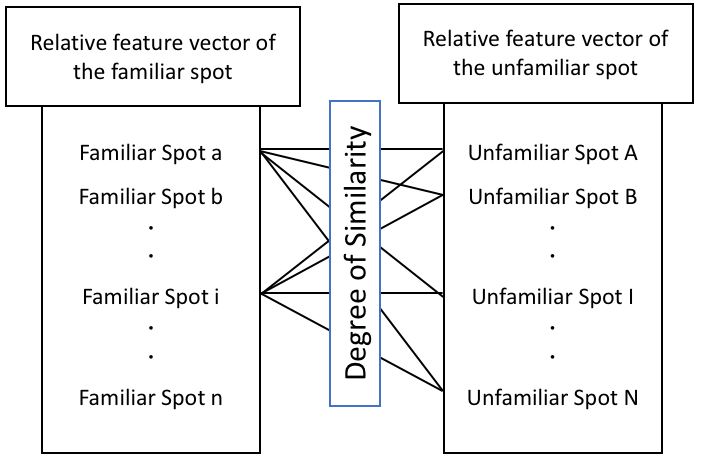
\includegraphics[clip,width=7.5cm,bb=0 0 720 540]{picture/Photo_CosSim_eng.png}
    % 類似度計算概念図
    \caption{Concept of similarity calculation}
    \label{fig:Photo_CosSim}
    \end{center}
\end{figure}

% 本研究では,観光スポットの特徴は相対的な特徴を利用する.
In this research, features of tourist spots make use of relative features.
% 相対的な特徴とは,特定の観光スポットが,ある観光スポット集合に含まれた他の観光スポットと比較した場合における独特な特徴である.
The relative feature is a unique feature when a specific tourist spot is compared with other tourist spots included in a set of tourist spots.
% 例として,観光スポット集合内に鹿苑寺と清水寺が存在する場合を考える.
As an example, consider the case where there are ``Rokuonji'' and ``Kiyomizudera'' in the tourist spot group.
% このとき鹿苑寺の特徴は,金色,金箔,輝き等となり,清水寺の特徴は,舞台,胎内,一望等となる.
At this time, the features of ``Rokuonji'' will be gold color, gold leaf, glow, etc., the features of ``Kiyomizudera'' are the stage, the womb inside, the panoramic view etc.
% どちらも京都に存在する寺院であるため,京都や寺院に関連する特徴は独特な特徴として現れることがない.
Because both are temples existing in Kyoto, features related to Kyoto and temples do not appear as unique features.
% 次に,観光スポット集合内に東京都庁舎展望台と鹿苑寺が存在する場合を考える.
Next, consider the case where ``the Tokyo Metropolitan Government Building Observatories'' and ``Rokuonji'' exist within the tourist spot group.
% このとき鹿苑寺の特徴は,金閣寺,お寺,金色,京都等となり,東京都庁舎の特徴は,展望,夜景,新宿等となる.
Features of ``Rokuonji'' at this time will be Kinkakuji, a temple, golden color, Kyoto etc.
% 観光スポットのカテゴリーが大きく異なる場合であれば,カテゴリーとしての特徴が現れる.
Features of ``the Tokyo Metropolitan Government Building Observatories'' will be perspectives, night view, Shinjuku etc.
% また,スポット自身の特徴を表すことができる.
If the categories of tourist spots are largely different, features as categories will appear.
% 本研究では,あるスポットが集合内の他のスポットと比較するとき,より各スポットの特徴を明らかにできる相対的な特徴に着目して研究を行う.
Also, it can show the features of the spot itself.
In this research, when a certain spot compares with other spots in the set, we focus on the relative features that make it possible to clarify the features of each spot.

% スポット差分ベクトルは式\ref{math:Vector difference}として定義される.
The spot differential vector is defined as formula \ref{math:Vector difference}.
% スポット差分ベクトルを求めるスポットを除いたスポット集合の各スポットのスポットベクトルの平均値を引いた値となる.
Is the value obtained by subtracting the average value of the spot vectors of the spots of the spot group excluding the spot for which the spot differential vector is found.
% $spot_{set} =\{s_1,s_2,\dots,s_i,\dots,s_n\}$は既訪問スポット集合や未訪問スポット集合となっている.
$spot_{set} =\{s_1,s_2,\dots,s_i,\dots,s_n\}$1 is an already visited spot set or an unvisited spot set.
% また,$s_i$は集合内のある観光スポットを示している.
$s_i$ is a tourist spot in the set.

\begin{equation}
  v_i=s_i-average(spot_{set}-s_i)
    \label{math:Vector difference}
\end{equation}


%%%%%%%%%%%%%%%%%%%%%%%%%%%%%%%%%%%%%%%%%%
%説明スポットの決定
\subsection{Determination of explainable spot}
\label{subsec:Determination of explainable spot}

% 既訪問スポットの各特徴差分ベクトル$v_i$と未訪問スポットの各特徴差分ベクトル$v_j$から,既訪問スポットと未訪問スポット間の相対的な特徴の類似度(図\ref{fig:photo_cossim})を求める.
From the feature difference vector $v_i$ of the visited spot and the feature difference vector $v_j$ of the unvisited spot, the relative feature similarity between the visited spot and the unvisited spot (Fig. \ref{fig:Photo_CosSim} ).
% 類似度計算には,コサイン尺度(式\ref{math:CosSim})を用いる.
For the similarity calculation, use the cosine scale (formula \ref{math:CosSim}).

\begin{eqnarray}
cos(v_i,v_j)=\frac{v_{i1}v_{j1}+v_{i2}v_{j2}+\cdots+v_{in}v_{jn}}
{\sqrt{v^2_{i1}+\cdots+v^2_{in}}\times\sqrt{v^2_{j1}+\cdots+v^2_{jn}}}
\label{math:CosSim}
\end{eqnarray}

% 既訪問スポットの各特徴ベクトルと未訪問エリア内の各特徴ベクトルの類似度が0.125以上かつ,類似度が最も高い既訪問スポットと未訪問スポットの関連付けを行う.
A correlation between the already visited spot having similarity of each feature vector of the already visited spot and each feature vector in the unvisited area of 0.125 or more and the highest similarity and the unvisited spot is performed.
% また,既訪問スポットと未訪問スポットとの関連をつけるとき以下の2つの方法がある.
In addition, there are two ways to establish an association between an already visited spot and an unvisited spot.

\begin{enumerate}
  % \item 既訪問スポットをベースにして未訪問スポットと関連付ける方法
  \item how to relate to unvisited spots based on already visited spots
  % \item 未訪問スポットをベースにして既訪問スポットと関連付ける方法
  \item how to relate to already visited spots based on unvisited spots
\end{enumerate}

% 方法1では,既訪問スポットをベースにすると未訪問エリア内のスポットが複数の特徴を保持する場合は同じ未訪問スポットと関連付ける場合がある.
In the method 1, if the spot in the unvisited area holds a plurality of features when using the already visited spot as the base, there are cases where the spot is associated with the same unvisited spot.
% 方法2では,未訪問スポットをベースにすることによって,既訪問スポット集合から各スポットの特徴を取り出し,未訪問スポットと関連付けることができるため,方法2を利用する.
In method 2, method 2 is used as it is possible to extract features of each spot from the already visited spot set based on the unvisited spot and associate with the unvisited spot.
% また,本研究では,未訪問スポットを説明するため未訪問スポットをベースにすることが妥当と考えられる.
In addition, in this research, it is considered reasonable to base on unvisited spots to explain unvisited spots.

%%%%%%%%%%%%%%%%%%%%%%%%%%%%%%%%%%%%%%%%%%
% 説明するための役割語の抽出
\subsection{Extraction of explainable words for role}
\label{subsec:Extraction of explainable words for role}
% 観光スポットのレビューはすべて形態素解析器「mecab-ipadic-NEologd」を使用することで,単語抽出処理を行う.
All tourist spots review words by using morphological analyzer ``mecab-ipadic-NEologd''.
% しかし,これらを用いて得られた単語は,日本語として成立しない語が含まれており,これらノイズの削除が必要となる.
However, words obtained by using these words contain words that do not hold Japanese, and it is necessary to delete these noises.
% 具体的には,助詞,助動詞,連体詞,記号を削除する.
Specifically, delete particles, auxiliary verbs, rentaishi, symbols.

% 節\ref{subsec:Determination of explainable spot}で関連付けした既訪問スポットと未訪問スポットの説明情報は単語形式でユーザに提示するため,ある観光スポットのレビュー集合を文書$i$とし,$i$に対する単語$j$が出現するスポット集合の出現回数を$TF_{i,j}$,単語$j$がスポット集合の文書数を$DF_{j}$,スポット集合内の全スポット数を$|D|$とした時,そのスポットにおける単語の特徴量は,式\ref{math:TFIDF}で定義される.
Since the explanation information of the visited spot and the unvisited spot associated in section \ref{subsec:Determination of explainable spot} is presented to the user in word format, a review set of a certain tourist spot is assumed to be a document $i$ and a spot where the word $j$ for $i$ appears When the number of occurrences of the set is $TF_{i,j}$, the word $j$ is the number of documents in the spot set is $DF_{j}$, and the total number of spots in the spot set is $|D|$ The feature quantity of a word in a spot is defined by the formula \ref{math:TFIDF}.

\begin{equation}
  word_{i,j} = TF_{i,j} \times IDF_{j}
  \label{math:TFIDF}
\end{equation}
\begin{equation}
  IDF_{j} = log(\frac{|D|}{DF_{j}})
  \label{math:IDF}
\end{equation}

% 本手法では,既訪問スポットに関して,ユーザが複数個のスポットを入力する.
In this method, for visited spots, the user inputs plurality of spots.
% それぞれのスポットの全レビューをまとめて1つの文書と見なし,それ以外のスポットの全レビューも文書とみなすことで,式\ref{math:TFIDF},\ref{math:IDF}によってTFIDF値を算出し,既訪問スポット毎の特徴語とする.
By considering all reviews of each spot as one document at a time and by considering all reviews of the other spots as documents, the TFIDF value is calculated by the formula \ref{math:TFIDF}, \ref{math:IDF}, and use it as the feature words for each spot in the unvisited area.

% 未訪問エリアに関して,ユーザがエリアを指定して入力する.
Regarding the unvisited area, the user designates an area and inputs it.
% エリア内のそれぞれのスポットの全レビューをまとめて1つの文書と見なし,それ以外のスポットの全レビューも文書とみなすことで,式\ref{math:TFIDF},\ref{math:IDF}によってTFIDF値を算出し,未訪問エリアのスポット毎の特徴語とする.
By considering all reviews of each spot in the area as one document and considering all reviews of the other spots as a document, the TFIDF value is calculated by the formula \ref{math:TFIDF}, \ref{math:IDF}, and use it as the feature words for each spot in the unvisited area.

% 関連付けした既訪問スポットと未訪問スポットの説明情報は,TFIDFで求めた各スポットの特徴語による調和平均を用いて決定する.
The explanation information on the associated visited spots and unvisited spots associated with each other is determined by using harmonic averages according to feature words of each spot obtained by TFIDF.
% 調和平均とは,逆数の算術平均の逆数である.
The harmonic mean is the reciprocal of the arithmetic mean of the reciprocal.
% 既訪問スポットのレビュー文書と,未訪問スポットのレビュー文書に,共通して出現する単語を抽出する.
Extracts commonly appearing words in the review document of the already visited spot and the review document of the unvisited spot.
% 抽出した単語のスコアは式\ref{math:Harmonic Mean}によって定義する.
The score of the extracted word is defined by the formula \ref{math:Harmonic Mean}.
% $word_{visited}$と$word_{unvisited}$は同じ単語がそれぞれ既訪問スポットのTFIDF値と未訪問スポットのTFIDF値を示している.
$word_{visited}$ and $word_{unvisited}$ indicate the TFIDF value of the visited spot and the TFIDF value of the unvisited spot, respectively.
% 単語スコアの値が大きと既訪問スポットと未訪問スポットのそれぞれのTFIDF値が大きい,つまり単語がそれぞれの文書に置いて重要度が高いことを示している.
When the value of the word score is large, the TFIDF value of each of the visited spot and the unvisited spot is large, that is, the word has high importance in each document.
% よって,単語スコアの上位10個の単語を説明情報としてユーザに提示する.
Therefore, the top ten words of the word score are presented to the user as explanation information.

\begin{eqnarray}
  score=\frac{1}{\frac{1}{2}(\frac{1}{word_{visited}}+\frac{1}{word_{unvisited}})}
  \label{math:Harmonic Mean}
\end{eqnarray}

%%%%%%%%%%%%%%%%%%%%%%%%%%%%%%%%%%%%%%%%%%
\subsection{Example of explained unfamiliar tourist spots}
\label{subsec:Example of explained unfamiliar tourist spots}




%%%%%%%%%%%%%%%%%%%%%%%%%%%%%%%%%%%%%%%%%%
%%%%%%%%%%%%%%%%%%%%%%%%%%%%%%%%%%%%%%%%%%
\section{Evaluation Experiment}
\label{sec:Evaluation Experiment}
%%%%%%%%%%%%%%%%%%%%%%%%%%%%%%%%%%%%%%%%%%
%%%%%%%%%%%%%%%%%%%%%%%%%%%%%%%%%%%%%%%%%%
\subsection{Experiment of feature word representing relation}
\label{subsec:Experiment of feature word representing relation}



\subsection{Comparative experiment of correspondence}
\label{subsec:Comparative experiment of correspondence}



%%%%%%%%%%%%%%%%%%%%%%%%%%%%%%%%%%%%%%%%%%
%%%%%%%%%%%%%%%%%%%%%%%%%%%%%%%%%%%%%%%%%%
\section{Conclusions and Future Work}
\label{sec:Conclusions and Future Work}
%%%%%%%%%%%%%%%%%%%%%%%%%%%%%%%%%%%%%%%%%%
%%%%%%%%%%%%%%%%%%%%%%%%%%%%%%%%%%%%%%%%%%



% use section* for acknowledgement
\section*{Acknowledgment}


The authors would like to thank...

The preferred spelling of the word "acknowledgment" in American
English is without an "e" after the "g." Use the singular heading
even if you have many acknowledgments. Avoid expressions such as
"One of us (S.B.A.) would like to thank ... ." Instead, write "F. A.
Author thanks ... ." Sponsor and financial support acknowledgments
are placed in the unnumbered footnote on the first page, not here.


% Can use something like this to put references on a page
% by themselves when using endfloat and the captionsoff option.
\ifCLASSOPTIONcaptionsoff
  \newpage
\fi



% trigger a \newpage just before the given reference
% number - used to balance the columns on the last page
% adjust value as needed - may need to be readjusted if
% the document is modified later
%\IAENGtriggeratref{8}
% The "triggered" command can be changed if desired:
%\IAENGtriggercmd{\enlargethispage{-5in}}

% references section

% can use a bibliography generated by BibTeX as a .bbl file
% BibTeX documentation can be easily obtained at:
% http://www.ctan.org/tex-archive/biblio/bibtex/contrib/doc/
% The IAENGtran BibTeX style support page is at:
% http://www.michaelshell.org/tex/IAENGtran/bibtex/
%\bibliographystyle{IAENGtran}
% argument is your BibTeX string definitions and bibliography database(s)
%\bibliography{IAENGabrv,../bib/paper}
%
% <OR> manually copy in the resultant .bbl file
% set second argument of \begin to the number of references
% (used to reserve space for the reference number labels box)
\begin{thebibliography}{1}
  \bibitem{Codd01}
    T. Kurashima, T. Iwata, G. Irie and K. Fujimura.,
      ``Travel route recommendation using geotags in photo sharing sites'',
      CIKM '10 Proceedings of the 19th ACM international conference on Information and knowledge management, pp.579-588, 2010
  \bibitem{Codd02}
    R. Kitamura and T. Itoh,
      ``Tourist Spot Recommmendation Applying Generic Object Recognition with Travel Photos'',
      ITE Tech. Rep., Vol.42, No.12, AIT2018-94, pp.185-188, 2018
  \bibitem{Codd03}
    A. J. Cheng, Y. Y. Chen, Y. T. Huang and Winston H. Hsu,
      ``Personalized Travel Recommendation by Mining People Attributes from Community-Contributed Photos'',
      MM '11 Proceedings of the 19th ACM international conference on Multimedia, pp.83-92, 2011
  \bibitem{Codd04}
    K. J. Holyoak and P. Thagard,
      ``Mental Leaps: Analogy in Creative Thought, MIT Press'',
      % Cambridge, 1995 %英語用
      Journal of Japanese Society for Artificial Intelligence,  Vol.11, No.3,  pp.489, 1996
  \bibitem{Codd05}
    D. Gentner,
      ``Structure-Mapping: A Theoretical Framework for Analogy'',
      Cognitive Science, Vol.7, pp.155–170, 1983
  \bibitem{Codd06}
    M. L. Gick and K. J. Holyoak,
      ``Analogical Problem Solving'',
      Cognitive Psychology, Vol.12, pp.306–355, 1980
  \bibitem{Codd07}
    M. L. Gick and K. J. Holyoak,
      ``Scheme Induction and Similarity in Analogical Transfer'',
      Cognitive Psychology, Vol.15, pp.1–38, 1983
  \bibitem{Codd08}
    Z. Chen and M. W. Daehler,
      ``Positive and Negative Transfer in Analogical Problem-solving by 6-years-old Children'',
      Cognitive Development, Vol.4, No.4, pp.327–344, 1989
  \bibitem{Codd09}
    K. J. Holyoak and P. Thagard,
      ``Analogical Mapping by Constraint Satisfaction'',
      Cognitive Science, Vol.13, pp.295–355, 1989
  \bibitem{Codd10}
    % 日本の形態素解析に条件付きランダムフィールドを適用する
    T. Kudo, K. Yamamoto and Y. Matsumoto,
    ``Applying Conditional Random Fields to Japanese Morphological Analysis'',
    Proceedings of the 2004 Conference on Empirical Methods in Natural Language Processing (EMNLP-2004), pp.230-237, 2004

\end{thebibliography}


\end{document}
